\documentclass[a4paper]{article}
\input{~/preamble.tex}

\title{Συστήματα Αναμονής, 5η εργαστηριακή άσκηση}
\author{Νικόλαος Παγώνας, el18175}
\date{}

\begin{document}
\maketitle

\section*{Δίκτυο με εναλλακτική δρομολόγηση}

\subsection*{(1)} 

Οι παραδοχές που πρέπει να κάνουμε προκειμένου οι σύνδεσμοι (γραμμές) να μπορούν να μοντελοποιηθούν σαν M/M/1 ουρές είναι: 

\begin{itemize}
	\item Οι εξωτερικές αφίξεις είναι ανεξάρτητες ροές Poisson.
	\item Έχουμε ανεξάρτητους εκθετικούς ρυθμούς εξυπηρέτησης $μ_i$.
	\item Η εσωτερική δρομολόγηση γίνεται με τυχαίο τρόπο.
	\item Οι χρόνοι εξυπηρέτησης πελατών χαρακτηρίζονται από έλλειψη μνήμης (Kleinrock's Independence Assumption)
	\item Έχουμε άπειρες FIFO ουρές, χωρίς απώλειες.
\end{itemize}

\subsection*{(2)}

Κάνοντας τις ανωτέρω παραδοχές, χρησιμοποιούμε το Octave για να σχεδιάσουμε το διάγραμμα μέσου χρόνου καθυστέρησης E(T) ενός τυχαίου πακέτου στο σύστημα συναρτήσει του α, (α = 0.001, 0.002, ..., 0.999):

\begin{figure}[H]
	\begin{center}
		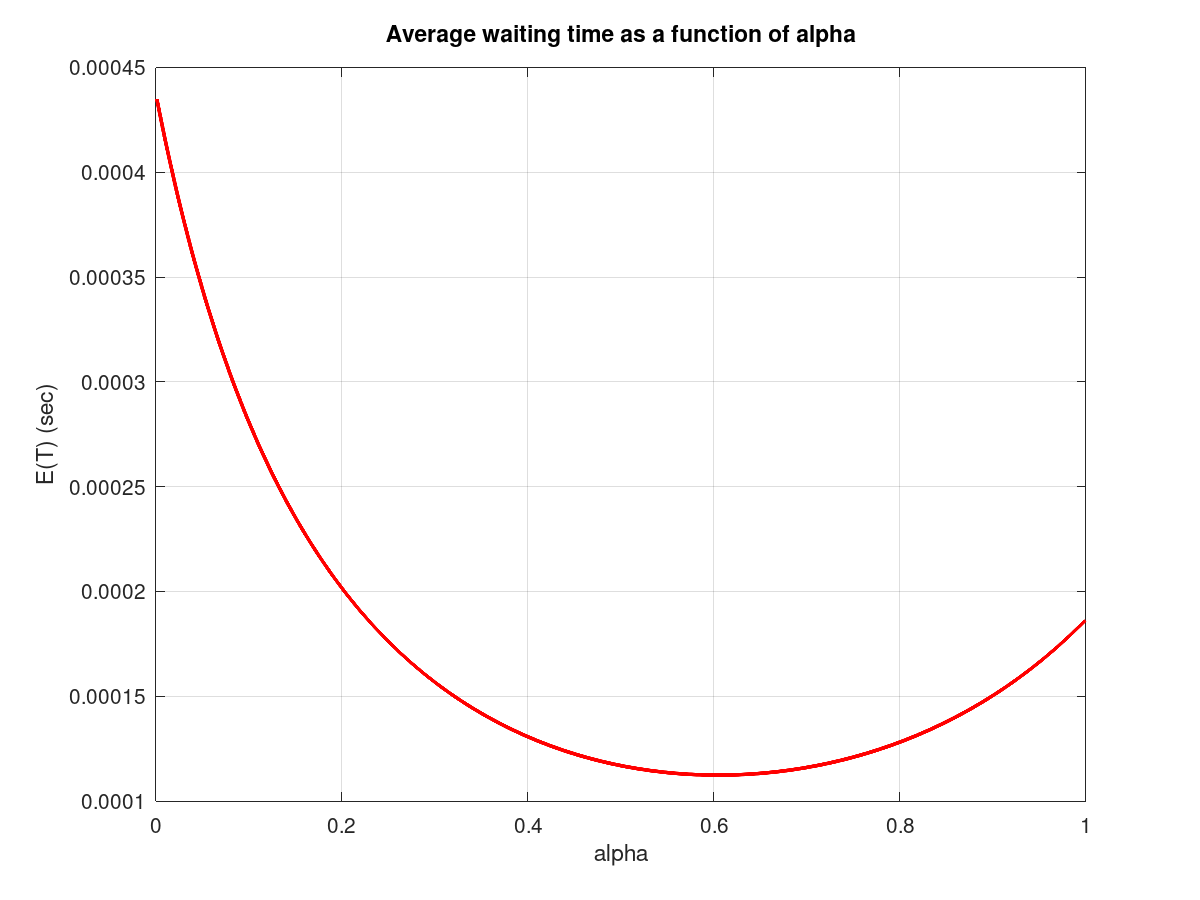
\includegraphics[width=0.7\textwidth]{two_lines.png}
	\end{center}
\end{figure} 

Για το παραπάνω διάγραμμα χρησιμοποιήθηκαν οι σχέσεις:

\begin{align*}
	λ_1 &= a \cdot λ \\
	λ_2 &= (1-a) \cdot λ \\
	ρ_1 &= \frac{λ_1}{μ_1} \\
	ρ_2 &= \frac{λ_2}{μ_2} \\
	E(n_1) &= \frac{ρ_1}{1-ρ_1} \\
	E(n_2) &= \frac{ρ_2}{1-ρ_2} \\
	E(n) &= E(n_1) + E(n_2) \\
	E(T) &= \frac{E(n)}{γ} = \frac{E(n)}{λ}
\end{align*}

Στη συνέχεια, υπολογίζουμε την τιμή του α που ελαχιστοποιεί το E(T), καθώς και τον ελάχιστο χρόνο καθυστέρησης E(T):

\verbatiminput{two_lines.txt}

\subsection*{Ο κώδικας που χρησιμοποιήθηκε}

\texttt{two\_lines.m}
\lstinputlisting[language=Octave]{two_lines.m}

\section*{Ανοιχτό δίκτυο ουρών αναμονής}

\subsection*{(1)}

Οι παραδοχές που πρέπει να κάνουμε ώστε το παραπάνω δίκτυο να μπορεί να μελετηθεί ως ανοιχτό δίκτυο με το θεώρημα Jackson είναι:

\begin{itemize}
	\item Οι εξωτερικές αφίξεις είναι ανεξάρτητες ροές Poisson.
	\item Έχουμε ανεξάρτητους εκθετικούς ρυθμούς εξυπηρέτησης $μ_i$.
	\item Η εσωτερική δρομολόγηση γίνεται με τυχαίο τρόπο.
	\item Οι χρόνοι εξυπηρέτησης πελατών χαρακτηρίζονται από έλλειψη μνήμης (Kleinrock's Independence Assumption)
	\item Έχουμε άπειρες FIFO ουρές, χωρίς απώλειες.
\end{itemize}

\begin{minipage}{\textwidth}
\subsection*{(2)}

Για τις ουρές $Q_1-Q_5$ έχουμε:

\begin{align*}
	ρ_1 &= \frac{λ_1}{μ_1} \\
	ρ_2 &= \frac{\dfrac{2}{7}\cdot λ_1+λ_2}{μ_2} \\
	ρ_3 &= \frac{\dfrac{4}{7}\cdot λ_1}{μ_3} \\
	ρ_4 &= \frac{\dfrac{1}{2}\cdot\dfrac{4}{7}\cdot λ_1+\dfrac{1}{7}\cdot λ_1}{μ_4} = \frac{\dfrac{3}{7}\cdot λ_1}{μ_4} \\
	ρ_5 &= \frac{\dfrac{1}{2}\cdot \dfrac{4}{7} \cdot λ_1 + \dfrac{2}{7} \cdot λ_1 + λ_2}{μ_5} = \frac{\dfrac{4}{7}λ_1 + λ_2}{μ_5} \\
\end{align*}

\end{minipage}

Η ζητούμενη συνάρτηση είναι υλοποιημένη στο αρχείο \texttt{intensities.m}

\lstinputlisting[language=Octave]{intensities.m}

\subsection*{(3)}

Η ζητούμενη συνάρτηση είναι υλοποιημένη στο αρχείο \texttt{mean\_clients.m}

\lstinputlisting[language=Octave]{mean_clients.m}

\begin{minipage}{\textwidth}
\subsection*{(4)}

Για τις τιμές των παραμέτρων που δίνονται, υπολογίζουμε την ένταση του φορτίου κάθε ουράς και τον μέσο χρόνο καθυστέρησης ενός πελάτη από άκρο σε άκρο του δικτύου:

\verbatiminput{network1.txt}

\end{minipage}

\subsection*{(5)}

Από το παραπάνω αποτέλεσμα, παρατηρούμε ότι το bottleneck του δικτύου (δηλαδή η ουρά με την μεγαλύτερη ένταση φορτίου) είναι η $Q_1$. Έτσι, για να παραμείνει το σύστημα εργοδικό, πρέπει και αρκεί να έχουμε $ρ_1 < 1$, δηλαδή $λ_1 < μ_1 = 6$.

\subsection*{(6)}

Για τις τιμές των παραμέτρων που δόθηκαν παραπάνω και για $λ_1$ από $ 0.1 \times 6 $ έως $ 0.99 \times 6 $, σχεδιάζουμε το διάγραμμα του μέσου χρόνου καθυστέρησης ενός πελάτη από άκρο σε άκρο του δικτύου:

\begin{figure}[H]
	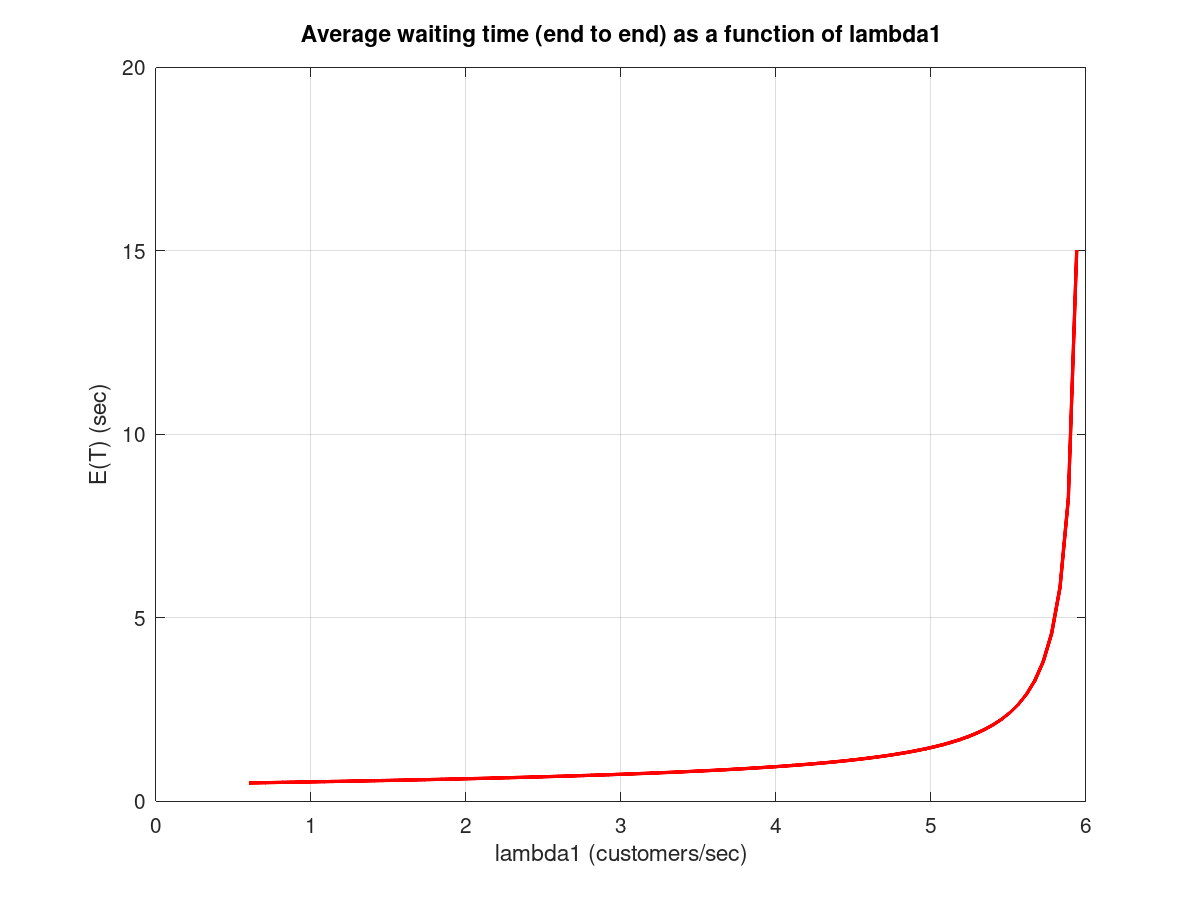
\includegraphics[width=\textwidth]{network.png}
\end{figure}

\subsection*{Ο κώδικας που χρησιμοποιήθηκε}

\texttt{network.m}
\lstinputlisting[language=Octave]{network.m}

\end{document}